\documentclass{report}
\usepackage{luatexja} % LuaTeXで日本語を使うためのパッケージ
\usepackage{luatexja-fontspec} % LuaTeX用の日本語フォント設定

% --- 数学関連 ---
\usepackage{amsmath, amssymb, amsfonts, mathtools, bm, amsthm} % 基本的な数学パッケージ
\usepackage{type1cm, upgreek} % 数式フォントとギリシャ文字
\usepackage{physics, mhchem} % 物理や化学の記号や式の表記を簡単にする

% --- 表関連 ---
\usepackage{multirow, longtable, tabularx, array, colortbl, dcolumn, diagbox} % 表のレイアウトを柔軟にする
\usepackage{tablefootnote, truthtable} % 表中に注釈を追加、真理値表
\usepackage{tabularray} % 高度な表組みレイアウト

% --- グラフィック関連 ---
\usepackage{tikz, graphicx} % 図の描画と画像の挿入
\usepackage{background} % ウォーターマークの設定
\usepackage{caption, subcaption} % 図や表のキャプション設定
\usepackage{float, here} % 図や表の位置指定

% --- レイアウトとページ設定 ---
\usepackage{fancyhdr} % ページヘッダー、フッター、余白の設定
\usepackage[top = 20truemm, bottom = 20truemm, left = 20truemm, right = 20truemm]{geometry}
\usepackage{fancybox, ascmac} % ボックスのデザイン

% --- 色とスタイル ---
\usepackage{xcolor, color, colortbl, tcolorbox} % 色とカラーボックス
\usepackage{listings, jvlisting} % コードの色付けとフォーマット

% --- 参考文献関連 ---
\usepackage{biblatex, usebib} % 参考文献の管理と挿入
\usepackage{url, hyperref} % URLとリンクの設定

% --- その他の便利なパッケージ ---
\usepackage{footmisc} % 脚注のカスタマイズ
\usepackage{multicol} % 複数段組
\usepackage{comment} % コメントアウトの拡張
\usepackage{siunitx} % 単位の表記
\usepackage{docmute}
% \usepackage{appendix}
% --- tcolorboxとtikzの設定 ---
\tcbuselibrary{theorems, breakable} % 定理のボックスと改ページ設定
\usetikzlibrary{decorations.markings, arrows.meta, calc} % tikzの装飾や矢印の設定

% --- 定理スタイルと数式設定 ---
\theoremstyle{definition} % 定義スタイル
\numberwithin{equation}{section} % 式番号をサブセクション単位でリセット

% --- hyperrefの設定 ---
\hypersetup{
  setpagesize = false,
  bookmarks = true,
  bookmarksdepth = tocdepth,
  bookmarksnumbered = true,
  colorlinks = false,
  pdftitle = {}, % PDFタイトル
  pdfsubject = {}, % PDFサブジェクト
  pdfauthor = {}, % PDF作者
  pdfkeywords = {} % PDFキーワード
}

% --- siunitxの設定 ---
\sisetup{
  table-format = 1.5, % 小数点以下の桁数
  table-number-alignment = center, % 数値の中央揃え
}

% --- 透かし画像の設定 --- 
\backgroundsetup{
  scale=0.5,                       % 画像のスケール
  % color=black,                   % 画像の色(透かし用に半透明が推奨)
  opacity=0.2,                   % 透かしの透明度(0が完全透明、1が完全不透明)
  angle=0,                       % 画像の角度
  position = current page.south east,  % ページの右下
  hshift=-6cm, % 右方向へのシフト(負の値で内側に移動)
  vshift=5cm,  % 上方向へのシフト(正の値で内側に移動)
  contents={
\includegraphics{./fig/appilogo-circular-full.png}} % 画像のパス
}

% --- その他の設定 ---
\allowdisplaybreaks % 数式の途中改ページ許可
\newcolumntype{t}{!{\vrule width 0.1pt}} % 新しいカラムタイプ
\newcolumntype{b}{!{\vrule width 1.5pt}} % 太いカラム
\UseTblrLibrary{amsmath, booktabs, counter, diagbox, functional, hook, html, nameref, siunitx, varwidth, zref} % tabularrayのライブラリ
\setlength{\columnseprule}{0.4pt} % カラム区切り線の太さ
\captionsetup[figure]{font = bf} % 図のキャプションの太字設定
\captionsetup[table]{font = bf} % 表のキャプションの太字設定
\captionsetup[lstlisting]{font = bf} % コードのキャプションの太字設定
\captionsetup[subfigure]{font = bf, labelformat = simple} % サブ図のキャプション設定
\setcounter{secnumdepth}{4} % セクションの深さ設定
\newcolumntype{d}{D{.}{.}{5}} % 数値のカラム
\newcolumntype{M}[1]{>{\centering\arraybackslash}m{#1}} % センター揃えのカラム
\DeclareMathOperator{\diag}{diag}
\everymath{\displaystyle} % 数式のスタイル
\newcommand{\inner}[2]{\left\langle #1, #2 \right\rangle}
\renewcommand{\figurename}{図}
\renewcommand{\i}{\mathrm{i}} % 複素数単位i
\renewcommand{\laplacian}{\grad^2} % ラプラシアンの記号
\renewcommand{\thesubfigure}{(\alph{subfigure})} % サブ図の番号形式
\newcommand{\m}[3]{\multicolumn{#1}{#2}{#3}} % マルチカラムのショートカット
\renewcommand{\r}[1]{\mathrm{#1}} % mathrmのショートカット
\newcommand{\e}{\mathrm{e}} % 自然対数の底e
\newcommand{\Ef}{E_{\mathrm{F}}} % フェルミエネルギー
\renewcommand{\c}{\si{\degreeCelsius}} % 摂氏記号
\renewcommand{\d}{\r{d}} % d記号
\renewcommand{\t}[1]{\texttt{#1}} % タイプライタフォント
\newcommand{\kb}{k_{\mathrm{B}}} % ボルツマン定数
% \renewcommand{\phi}{\varphi} % ϕをφに変更
\renewcommand{\epsilon}{\varepsilon}
\newcommand{\fullref}[1]{\textbf{\ref{#1} \nameref{#1}}}
\newcommand{\reff}[1]{\textbf{図\ref{#1}}} % 図参照のショートカット
\newcommand{\reft}[1]{\textbf{表\ref{#1}}} % 表参照のショートカット
\newcommand{\refe}[1]{\textbf{式\eqref{#1}}} % 式参照のショートカット
\newcommand{\refp}[1]{\textbf{コード\ref{#1}}} % コード参照のショートカット
\renewcommand{\lstlistingname}{コード} % コードリストの名前
\renewcommand{\theequation}{\thesection.\arabic{equation}} % 式番号の形式
\renewcommand{\footrulewidth}{0.4pt} % フッターの線
\newcommand{\mar}[1]{\textcircled{\scriptsize #1}} % 丸囲み文字
\newcommand{\combination}[2]{{}_{#1} \mathrm{C}_{#2}} % 組み合わせ
\newcommand{\thline}{\noalign{\hrule height 0.1pt}} % 細い横線
\newcommand{\bhline}{\noalign{\hrule height 1.5pt}} % 太い横線

% --- カスタム色定義 ---
\definecolor{burgundy}{rgb}{0.5, 0.0, 0.13} % バーガンディ色
\definecolor{charcoal}{rgb}{0.21, 0.27, 0.31} % チャコール色
\definecolor{forest}{rgb}{0.0, 0.35, 0} % 森の緑色

% --- カスタム定理環境の定義 ---
\newtcbtheorem[number within = chapter]{myexc}{練習問題}{
  fonttitle = \gtfamily\sffamily\bfseries\upshape,
  colframe = forest,
  colback = forest!2!white,
  rightrule = 1pt,
  leftrule = 1pt,
  bottomrule = 2pt,
  colbacktitle = forest,
  theorem style = standard,
  breakable,
  arc = 0pt,
}{exc-ref}
\newtcbtheorem[number within = chapter]{myprop}{命題}{
  fonttitle = \gtfamily\sffamily\bfseries\upshape,
  colframe = blue!50!black,
  colback = blue!50!black!2!white,
  rightrule = 1pt,
  leftrule = 1pt,
  bottomrule = 2pt,
  colbacktitle = blue!50!black,
  theorem style = standard,
  breakable,
  arc = 0pt
}{proposition-ref}
\newtcbtheorem[number within = chapter]{myrem}{注意}{
  fonttitle = \gtfamily\sffamily\bfseries\upshape,
  colframe = yellow!20!black,
  colback = yellow!50,
  rightrule = 1pt,
  leftrule = 1pt,
  bottomrule = 2pt,
  colbacktitle = yellow!20!black,
  theorem style = standard,
  breakable,
  arc = 0pt
}{remark-ref}
\newtcbtheorem[number within = chapter]{myex}{例題}{
  fonttitle = \gtfamily\sffamily\bfseries\upshape,
  colframe = black,
  colback = white,
  rightrule = 1pt,
  leftrule = 1pt,
  bottomrule = 2pt,
  colbacktitle = black,
  theorem style = standard,
  breakable,
  arc = 0pt
}{example-ref}
\newtcbtheorem[number within = chapter]{exc}{Requirement}{myexc}{exc-ref}
\newcommand{\rqref}[1]{{\bfseries\sffamily 練習問題 \ref{exc-ref:#1}}}
\newtcbtheorem[number within = chapter]{definition}{Definition}{mydef}{definition-ref}
\newcommand{\dfref}[1]{{\bfseries\sffamily 定義 \ref{definition-ref:#1}}}
\newtcbtheorem[number within = chapter]{prop}{命題}{myprop}{proposition-ref}
\newcommand{\prref}[1]{{\bfseries\sffamily 命題 \ref{proposition-ref:#1}}}
\newtcbtheorem[number within = chapter]{rem}{注意}{myrem}{remark-ref}
\newcommand{\rmref}[1]{{\bfseries\sffamily 注意 \ref{remark-ref:#1}}}
\newtcbtheorem[number within = chapter]{ex}{例題}{myex}{example-ref}
\newcommand{\exref}[1]{{\bfseries\sffamily 例題 \ref{example-ref:#1}}}
% --- 再定義コマンド ---
% \mathtoolsset{showonlyrefs=true} % 必要な式番号のみ表示
\pagestyle{fancy} % ヘッダー・フッターのスタイル設定
\chead{応用量子物性講義ノート} % 中央ヘッダー
% \rhead{}
\fancyhead[R]{\rightmark}
\renewcommand{\sectionmark}[1]{\markright{\thesection\ #1}}
\cfoot{\thepage} % 中央フッターにページ番号
\lhead{}
\rfoot{Yuto Masuda and Haruki Aoki} % 右フッターに名前
\setcounter{tocdepth}{4} % 目次の深さ
\makeatletter
\@addtoreset{equation}{section} % サブセクションごとに式番号をリセット
\makeatother

% --- メタ情報 ---
\title{応用量子物性講義ノート}
\date{更新日\today}
\author{Yuto Masuda and Haruki Aoki}

\begin{document}
  本節では量子力学的に散乱を議論する.量子力学では波動関数を用いて散乱体の様子を調べる.
  まず,散乱帯のポテンシャルを紹介して,散乱振幅$f(\theta)$を求めればいいことを知る.
  次に,散乱振幅と微分断面積の関係を調べる.
  最後に,具体的に散乱振幅の表式を導く.
  \subsection{散乱振幅}
    散乱体が球対称ポテンシャル$V(r)$を持つとする.Schrödinger方程式は
    \begin{align}
      \qty(-\frac{\hbar^2}{2m}\laplacian + V(r))\psi(\bm{r}) = E \psi(\bm{r})\label{se-scattering}
    \end{align}
    である.
    ここで,$V(r)$は$r \to \infty$で$r^{-1}$より早く$V \to 0$となるとする.
    なお,$r \to \infty$で$r^{-1}$より早く$0$に収束することを,十分早く収束するということにする.
    $z$軸に沿う入射波は平面波なので,
    \begin{align}
      \psi_{\r{in}} = \e^{\i k z}\ (z \to \infty)
    \end{align}
    と表せる.
    また,散乱波は外向きの球面波となるので,
    \begin{align}
      \psi_{\r{sc}} \simeq \frac{\e^{\i kr}}{r}\ (r \to \infty)
    \end{align}
    である.散乱問題とは,$r \to \infty$で
    \begin{align}
      \psi(\bm{r}) &= \psi_{\r{in}} + \psi_{\r{sc}} \\ 
      &= \e^{\i kz} + f(\theta) \frac{\e^{\i kr}}{r}
    \end{align}
    を満たす\refe{se-scattering}の定常解を求めることである.$f(\theta)$を散乱振幅という.上式は重要なので強調しておく.
    \begin{itembox}[l]{散乱問題の境界条件}
      \begin{equation}
        \psi(\bm{r}) = \e^{\i kz} + f(\theta) \frac{\e^{\i kr}}{r}
      \end{equation}
    \end{itembox}
  \subsection{散乱振幅と微分断面積の関係}
    この問題を解くための準備として確率密度$\rho \coloneqq \psi^{*} \psi$の時間変化を考える.
    時間変化するSchr\"odinger方程式より,
    \begin{align}
      \i\hbar\pdv{\psi}{t} &= \hat{H}\psi \\ 
      \Leftrightarrow \pdv{\psi}{t} &= \frac{1}{\i\hbar}\hat{H}\psi \\ 
      \Leftrightarrow \pdv{\psi^*}{t} &= -\frac{1}{\i\hbar}\hat{H}\psi^*
    \end{align}
    であることを用いると,
    \begin{align}
      \pdv{t}\rho &= \pdv{t}(\psi^{*}\psi) \\
      &= \pdv{\psi^*}{t}\psi + \psi^{*}\pdv{\psi}{t} \\
      &= -\frac{1}{\i\hbar}\qty[\qty(-\frac{\hbar^2}{2m}\laplacian + V)\psi^{*}]\psi + \psi^{*}\frac{1}{\i\hbar}\qty[\qty(-\frac{\hbar^2}{2m}\laplacian + V)\psi] \\
      &= \frac{\hbar}{2\i m}\qty[\qty(\laplacian \psi^{*})\psi - \psi^{*}\qty(\laplacian\psi)] \\
      &= -\frac{\hbar}{2\i m}\div \qty(\psi^{*}\grad\psi - \psi \grad\psi^{*})\label{prob-density}
    \end{align}
    確率流密度を,
    \begin{align}
      \bm{j} &\coloneqq \frac{\hbar}{2\i m} \qty(\psi^{*}\grad\psi - \psi \grad\psi^{*})\label{prob-flow} \\
      &= \frac{\hbar}{m}\Im \qty(\psi^{*}\grad\psi)
    \end{align}
    と定義する.
    \refe{prob-flow}を\refe{prob-density}に代入すると,確率密度に対する連続の式である,
    \begin{align}
      \pdv{t} \rho = -\div\bm{j}
    \end{align}
    を得る\footnote{両辺に電荷をかければ電荷保存の法則となる. }.
    \par
    次に微分断面積と散乱振幅の関係を考える.
    $z$軸に平行に入射しているので入射波は,
    \begin{align}
      \psi_{\r{in}} = \e^{\i kz}
    \end{align}
    と書けるのであった.
    入射波は$z$軸方向にしか存在しないので,その確率流密度の$z$成分$j_z$は\refe{psi-in-grad}より,
    \begin{align}
      j_z &= \frac{\hbar}{m}\Im \qty(\psi^{*}\pdv{z}\psi) \\ 
      &= \frac{\hbar}{m} \Im \qty(\e^{-\i kz} \i k e^{\i kz}) \\
      &= \frac{\hbar k}{m}
    \end{align}% メモ: 図にr軸を追加する.
    である.
    \par
    散乱波は,
    \begin{align}
      \psi_{\r{sc}} = \frac{f(\theta)}{r}\e^{\i kr}
    \end{align}
    と書けるのであった.
    散乱波は$r$軸方向にしか存在しないので,その確率流密度の$r$成分$j_r(\theta)$は,
    \begin{align}
      j_r(\theta) &= \frac{\hbar}{m}\Im \qty(\psi^{*}_{\r{sc}}\pdv{r}\psi_{\r{sc}}) \\
      &= \frac{\hbar}{m} \Im \qty[\frac{f(\theta)^*}{r} \e^{-\i kr}\qty(\frac{\i k}{r} - \frac{1}{r^2})f(\theta)\e^{\i kr}] \\
      &= \frac{\hbar}{m} \Im \qty[-\frac{\abs{f(\theta)}^2}{r^3} + \i k\frac{\abs{f(\theta)}^2}{r^2}] \\
      &= \frac{\hbar}{m} k\frac{\abs{f(\theta)}^2}{r^2} \\
      &= \frac{\abs{f(\theta)}^2}{r^2}j_z
    \end{align}
    である.
    \par
    さて,微分断面積と散乱振幅の関係について考えよう.
    微分断面積と粒子数の関係の両辺を$n$で割ると,
    \begin{align}
      \dd{N} &= \sigma (\theta) n \dd{\Omega} \\ 
      \Leftrightarrow \frac{\dd{N}}{n} &= \sigma (\theta) \dd{\Omega}
    \end{align}
    となる.$\frac{\dd{N}}{n}$は,
    \begin{align}
      \frac{\dd{N}}{n} &= \frac{\qty(\text{単位時間に位置$(r,\theta)$にある$検出器\dd{S}$に入射する粒子数})}{\qty(\text{単位時間単位面積当たりの入射粒子数})} \\ 
      &= \frac{\qty(\text{単位時間に位置$(r,\theta)$にある検出器$\dd{S}$に粒子が入射する確率})}{\qty(\text{単位時間単位面積当たりに粒子が入射する確率})} \\ 
      &= \frac{j_r \dd{S}}{j_z}
    \end{align}
    と書けるので,
    \begin{align}
      \sigma(\theta)\dd{\Omega} = \abs{f(\theta)}^2\frac{\dd{S}}{r^2}
    \end{align}
    が得られる.
    \refe{solid-angle-def}より,$\dd{\Omega} = \frac{\dd{S}}{r^2}$であるから,
    \begin{align}
      \sigma(\theta) = \abs{f(\theta)}^2
    \end{align}
    という関係が成り立つ.これは,散乱振幅から微分断面積が求められることを意味する.
    \begin{itembox}[l]{散乱振幅と微分断面積の関係}
      \begin{align}
        \sigma(\theta) = \abs{f(\theta)}^2
      \end{align}
    \end{itembox}
  \subsection{散乱振幅の表式}
    最後に散乱振幅$f(\theta)$の表式を求める.
    散乱のSchrödinger方程式は,
    \begin{align}
      \qty(-\frac{\hbar^2}{2m}\laplacian + V(r))\psi(\bm{r}) = E\psi(\bm{r})
    \end{align}
    であった.
    $\kappa$,$U(\bm{r})$を,
    \begin{align}
        \kappa &\coloneqq \frac{\sqrt{2mE}}{\hbar} \\
        U(\bm{r}) &\coloneqq \frac{2m}{\hbar^2} V(\bm{r})
    \end{align}
    と定義すると,
    \begin{align}
      \qty(\laplacian + \kappa^2)\psi(\bm{r}) = U(\bm{r}) \psi(\bm{r}) \label{helmholtz-eq}
    \end{align}
    と表せる.\refe{helmholtz-eq}の解は,Helmholtz方程式型の斉次式,
    \begin{align}
      \qty(\laplacian + \kappa^2)\phi(\bm{r}) = 0
    \end{align}
    の$z$方向に入射した場合の一般解$\phi(\bm{r}) = \e^{\i kz}$と,
    非斉次の方程式,
    \begin{align}
      \qty(\laplacian + \kappa^2)\chi(\bm{r}) = U(\bm{r}) \chi(\bm{r})\label{particular-solution}
    \end{align}
    の解となる$\chi(\bm{r})$の和である.
    \par
    では,\refe{particular-solution}の特解を求めよう.レシピはこうである.
    \begin{enumerate}
      \item $\qty(\laplacian + \kappa^2)G_0(\bm{r}) = \delta(\bm{r})$を満たすGreen関数$G_0$を求める.
      \item $\chi(\bm{r}) = \int\dd{\bm{r'}} G_0(\bm{r} - \bm{r'}) U(\bm{r'}) \psi(\bm{r'})$から特解を求める.
    \end{enumerate}
    2. から特解が求められるのは,
    \begin{align}
      \qty(\laplacian + \kappa^2)\chi(\bm{r}) &= \int \dd{\bm{r'}}\qty(\laplacian + \kappa^2)G_0(\bm{r} - \bm{r'}) U(\bm{r'}) \psi(\bm{r'}) \\
      &= \int\dd{\bm{r'}} \delta(\bm{r} - \bm{r'}) U(\bm{r'}) \psi(\bm{r'}) \\
      &= U(\bm{r}) \psi(\bm{r})
    \end{align}
    が成り立つからだ.
    \par
    まず,1. で定義したGreen関数の関係式,
    \begin{align}
      \qty(\laplacian + \kappa^2)G_0(\bm{r}) = \delta(\bm{r})
    \end{align}
    の両辺をFourier変換すると,
    \begin{align}
      \int\dd{\bm{r}} \qty(\laplacian + \kappa^2) G_0(\bm{r}) \e^{-\i\bm{k} \cdot \bm{r}} &= \int\dd{\bm{r}} \delta(\bm{r})\e^{-\i\bm{k}\cdot\bm{r}} \\
      \Leftrightarrow \qty[(-\i\bm{k})^2 + \kappa^2] \int\dd{\bm{r}} G_0(\bm{r}) \e^{-\i \bm{k}\cdot \bm{r}} &= 1
    \end{align}
    となる.Green関数$G_0(\bm{r})$のFourier変換を$\tilde{G}_0(\bm{k})$と書くと,
    \begin{align}
      \tilde{G}_0(\bm{k}) = \frac{1}{\kappa^2 - k^2}
    \end{align}
    を得る.よってGreen関数は$\tilde{G}_0(\bm{k})$を逆Fourier変換して,
    \begin{align}
      G_0(\bm{r}) &= \frac{1}{(2\pi)^3}\int\dd{\bm{k}} \frac{\e^{\i\bm{k} \cdot \bm{r}}}{\kappa^2 - k^2}\label{g-tilde-to-gr}
    \end{align}
    と表される.極座標に変換して\refe{g-tilde-to-gr}の積分を実行すると,
    \begin{align}
      G_0(\bm{r}) &=  \frac{1}{(2\pi)^3}\int\dd{\bm{k}}\frac{\e^{\i\bm{k} \cdot \bm{r}}}{\kappa^2 - k^2}\\ 
      &= \frac{1}{(2\pi)^3} \int\dd{\bm{k}} \frac{\exp\qty(\i kr\cos\theta)}{\kappa^2 - k^2} \\ 
      &= \frac{1}{(2\pi)^3} \int_{\phi = 0}^{2\pi}\dd{\phi}\int_{k = 0}^{\infty}\dd{k}\int_{\theta = 0}^{\pi}\dd{\theta} \frac{\exp(\i kr \cos \theta)}{\kappa^2 - k^2} k^2\sin\theta \\
      &= \frac{1}{(2\pi)^3} 2\pi \int_{k = 0}^{\infty} k^2 \dd{k} \int_{\theta = 0}^{\pi}\dd{\theta} \sin\theta\frac{\exp(\i k r\cos\theta)}{\kappa^2 - k^2} \\
      &= \frac{1}{(2\pi)^2} \int_{0}^{\infty}k^2\frac{\e^{\i kr} - \e^{-\i kr}}{\i kr\qty(\kappa^2 - k^2)}\dd{k} \\
      &= \frac{1}{4\pi^2\i r} \int_{0}^{\infty}k \frac{\e^{\i kr} - \e^{-\i kr}}{(\kappa - k)(\kappa + k)}\dd{k} \\
      &= \frac{1}{8\pi^2\i r} \int_{-\infty}^{\infty}k \frac{\e^{\i kr} - \e^{-\i kr}}{(\kappa - k)(\kappa + k)}\dd{k} \\
      &= \frac{1}{8\pi^2\i r} \int_{-\infty}^{\infty}k \qty[\frac{\e^{\i kr}}{(\kappa - k)(\kappa + k)} - \frac{\e^{-\i kr}}{(\kappa - k)(\kappa + k)}]\dd{k} \\ 
      &= \frac{\i}{8\pi^2 r} \int_{-\infty}^{\infty}k \qty[\frac{\e^{\i kr}}{(k - \kappa)(k + \kappa)} - \frac{\e^{-\i kr}}{(k - \kappa)(k + \kappa)}]\dd{k} \\ 
      &= \frac{\i}{4\pi^2 r}I
    \end{align}
    となる.ただし,$I$は,
    \begin{align}
      I \coloneqq \int_{-\infty}^{\infty} \frac{k \e^{\i kr}}{(k - \kappa)(k + \kappa)} \dd{k}
    \end{align}
    である.
    式変形の途中で,
    \begin{align}
      -\int_{-\infty}^{\infty}k \frac{\e^{-\i kr}}{(k - \kappa)(k + \kappa)}\dd{k} &= -\int_{\infty}^{-\infty}\qty(-k) \frac{\e^{-\i \qty(-k)r}}{\qty(\qty(-k) - \kappa)\qty(\qty(-k) + \kappa)}\qty(-\dd{k}) \\ 
      &= \int_{-\infty}^{\infty}k \frac{\e^{\i kr}}{(k - \kappa)(k + \kappa)}\dd{k} = I
    \end{align}
    なる関係を用いた.
    $I$を計算するには留数定理を用いる.
    \begin{itembox}[l]{留数定理}
      複素関数$f(z)$が閉経路$C$内に$m$個の特異点$b_1, \cdots b_m$を持つとすると,
      \begin{align}
        \oint_C f(z) \dd{z} = 2\pi\i\sum_{k = 1}^{m}\r{Res}\qty(b_k; f)
      \end{align}
      が成立する.
    \end{itembox}
    今回の場合は特異点は$\kappa$と$-\kappa$である.
    しかし,極の避け方にはいくつかのパターンがあり,それに応じてGreen関数の計算結果は複数存在する.
    これは何ら不自然なことではない.
    今計算しているのは,$\qty(\laplacian + \kappa^2)$なる演算子の固有関数$G_0$を求めているので,複数存在してもよい.
    まず,\reff{Integral}のように$-\kappa$を上に避け,$\kappa$を下に避けると,
    積分経路$C$で囲まれている領域に存在する特異点は,$k = \kappa$のみであるので,
    \begin{align}
      I &= \int_{-\infty}^{\infty} \frac{k \e^{\i kr}}{(k - \kappa)(k + \kappa)} \dd{k} \\ 
      &= 2\pi\i\frac{\e^{\i\kappa r}}{2} \\ 
      &= \pi\i\e^{\i\kappa r}
    \end{align}
    となるから,
    \begin{align}
      G_0(\bm{r}) &= \frac{\i}{4\pi^2 r}I \\ 
      &= -\frac{\e^{\i\kappa r}}{4\pi r}
    \end{align}
    となる\footnote{
      積分経路$C$に$-\kappa$と$\kappa$がそれぞれ含まれるか否かを分類して求めたGreen関数は,
      \begin{align*}
        G_0(\bm{r}) = 
        \begin{dcases}
          \text{不適} & $-\kappa$: 含まない,$\kappa$: 含まない \\ 
          \frac{\e^{\i\kappa r}}{4\pi r} & $-\kappa$: 含まない,$\kappa$: 含む \\ 
          \frac{\e^{-\i\kappa r}}{4\pi r} & $-\kappa$: 含む,$\kappa$: 含まない \\ 
          \i\frac{\sin\qty(\kappa r)}{4\pi r} & $-\kappa$: 含む,$\kappa$: 含む
        \end{dcases}
      \end{align*}
      $-\kappa$と$\kappa$をともに含まない経路で計算したとき,$I = 0$となるが,固有関数は0であってはいけないから,不適である.
    }.
    計算しているのは,外向き球面波解であるため,\reff{Integral}で示した経路で積分した結果が最も合理的であるから,このGreen関数を採用して以下の計算を行う.
    Green関数を用いると\refe{se-scattering}の形式解は,
    \begin{align}
      \psi(\bm{r}) &= \phi(\bm{r}) + \chi(\bm{r}) \\ 
      &= \e^{\i kz} + \int\dd{\bm{r'}} G_0(\bm{r} - \bm{r'}) U(\bm{r'}) \phi(\bm{r'}) \\ 
      &= \e^{\i kz} - \int \frac{\e^{\i\kappa \abs{\bm{r} - \bm{r'}}}}{4\pi \abs{\bm{r} - \bm{r'}}} \cdot \frac{2m}{\hbar^2} V(\bm{r'}) \cdot \psi(\bm{r'}\dd{\bm{r'}}) \\ 
      &= \e^{\i kz} - \frac{1}{4\pi} \int \frac{\e^{\i \kappa \abs{\bm{r} - \bm{r'}}}}{\abs{\bm{r} - \bm{r'}}} \frac{2m}{\hbar^2}V(r')\psi(\bm{r'}) \dd{\bm{r'}}\label{formal-soultion}
    \end{align}
    である.
    \begin{figure}[H]
      \centering
      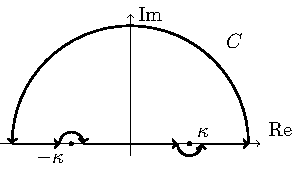
\includegraphics[width = 0.7\columnwidth]{fig/integral-green-tex.pdf}
      \caption{積分経路}\label{Integral}
    \end{figure}
    \par
    次に\refe{formal-soultion}から散乱振幅$f(\theta)$を求める.$V(r')$は$r' < a$でのみ$V\neq 0$であると仮定する.
    \reff{formal-soultion}において
    $r \gg r'$では,
    \begin{align}
      \abs{\bm{r} - \bm{r'}} &= \sqrt{r^2 - 2\bm{r} \cdot \bm{r'} + r'^2} \\
      &= r \qty[1 - \frac{2\bm{r}\cdot\bm{r'}}{r^2} + \qty(\frac{r'}{r})^2]^{1/2} \\
      &\simeq r - \bm{n}\cdot\bm{r'}\label{abs-r-r-prime-approx}
    \end{align}
    が成り立つ.よって,
    \begin{align}
      \e^{\i \kappa \abs{\bm{r} - \bm{r'}}} &\simeq \e^{\i \kappa \qty(r - \bm{n} \cdot \bm{r'})}\\
      &= \e^{\i \kappa r} - \e^{-\i \bm{\kappa} \cdot \bm{r'}}\label{exp-abs-r-r-prime-approx}
    \end{align}
    と近似できる.ただし,$\bm{\kappa} \coloneqq \kappa \bm{n}$を$z$軸と角度$\theta$をなす散乱方向の波数ベクトルとする.
    また,
    \begin{align}
      \frac{1}{\abs{\bm{r} - \bm{r'}}} &= \frac{1}{r}\qty[1 - \frac{2\bm{r}\cdot\bm{r'}}{r^2} + \qty(\frac{r'}{r})^2]^{-1/2} \\ 
      &\simeq \frac{1}{r}\label{abs-r-r-prime-inv-approx}
    \end{align}
    と近似する.% なぜ???
    \refe{exp-abs-r-r-prime-approx}や\refe{abs-r-r-prime-inv-approx}で行った近似結果を\refe{formal-soultion}に代入すると,
    \begin{align}
      \psi(\bm{r}) = \e^{\i kz} - \qty(\frac{1}{4\pi} \int \e^{-\i\bm{\kappa'}\cdot \bm{r'}} \frac{2m}{\hbar^2}V(r')\psi(\bm{r'})\dd{\bm{r'}})\frac{\e^{\i\kappa r}}{r}
    \end{align}
    である.したがって,散乱振幅は
    \begin{align}
      f(\theta) = -\frac{1}{4\pi} \int \dd{\bm{r'}} \e^{- \i \bm{\kappa'} \cdot \bm{r'}} \frac{2m}{\hbar^2}V(r')\psi(\bm{r'})
    \end{align}
    となる.
\end{document}
